% Created by tikzDevice version 0.7.0 on 2015-04-17 14:29:37
% !TEX encoding = UTF-8 Unicode
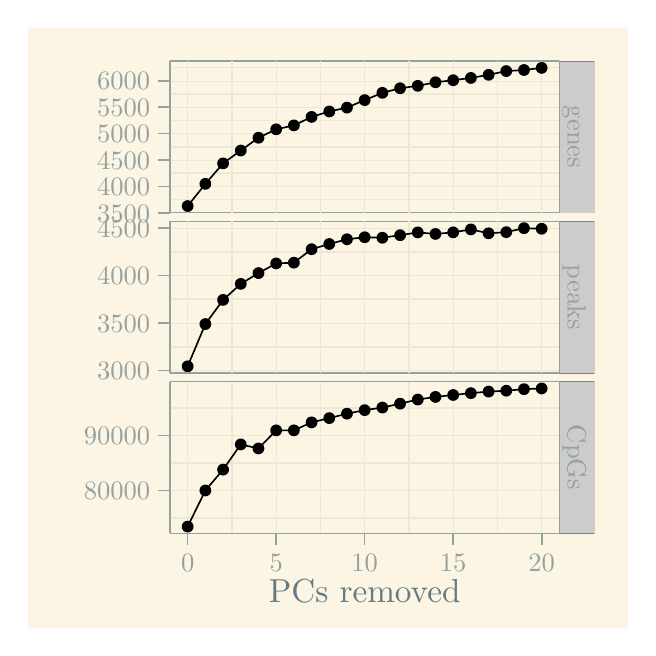
\begin{tikzpicture}[x=1pt,y=1pt]
\definecolor[named]{fillColor}{rgb}{0.99,0.96,0.89}
\path[use as bounding box,fill=fillColor] (0,0) rectangle (216.81,216.81);
\begin{scope}
\path[clip] (  0.00,  0.00) rectangle (216.81,216.81);

\path[fill=fillColor] (  0.00,  0.00) rectangle (216.81,216.81);
\end{scope}
\begin{scope}
\path[clip] ( 51.42,149.86) rectangle (192.13,204.77);
\definecolor[named]{drawColor}{rgb}{0.58,0.63,0.63}
\definecolor[named]{fillColor}{rgb}{0.99,0.96,0.89}

\path[draw=drawColor,line width= 0.6pt,line join=round,line cap=round,fill=fillColor] ( 51.42,149.86) rectangle (192.13,204.77);
\definecolor[named]{drawColor}{rgb}{0.93,0.91,0.84}

\path[draw=drawColor,line width= 0.6pt,line join=round] ( 51.42,154.67) --
	(192.13,154.67);

\path[draw=drawColor,line width= 0.6pt,line join=round] ( 51.42,164.21) --
	(192.13,164.21);

\path[draw=drawColor,line width= 0.6pt,line join=round] ( 51.42,173.75) --
	(192.13,173.75);

\path[draw=drawColor,line width= 0.6pt,line join=round] ( 51.42,183.29) --
	(192.13,183.29);

\path[draw=drawColor,line width= 0.6pt,line join=round] ( 51.42,192.83) --
	(192.13,192.83);

\path[draw=drawColor,line width= 0.6pt,line join=round] ( 51.42,202.36) --
	(192.13,202.36);

\path[draw=drawColor,line width= 0.6pt,line join=round] ( 73.80,149.86) --
	( 73.80,204.77);

\path[draw=drawColor,line width= 0.6pt,line join=round] (105.78,149.86) --
	(105.78,204.77);

\path[draw=drawColor,line width= 0.6pt,line join=round] (137.76,149.86) --
	(137.76,204.77);

\path[draw=drawColor,line width= 0.6pt,line join=round] (169.74,149.86) --
	(169.74,204.77);

\path[draw=drawColor,line width= 0.2pt,line join=round] ( 51.42,149.90) --
	(192.13,149.90);

\path[draw=drawColor,line width= 0.2pt,line join=round] ( 51.42,159.44) --
	(192.13,159.44);

\path[draw=drawColor,line width= 0.2pt,line join=round] ( 51.42,168.98) --
	(192.13,168.98);

\path[draw=drawColor,line width= 0.2pt,line join=round] ( 51.42,178.52) --
	(192.13,178.52);

\path[draw=drawColor,line width= 0.2pt,line join=round] ( 51.42,188.06) --
	(192.13,188.06);

\path[draw=drawColor,line width= 0.2pt,line join=round] ( 51.42,197.59) --
	(192.13,197.59);

\path[draw=drawColor,line width= 0.2pt,line join=round] ( 57.81,149.86) --
	( 57.81,204.77);

\path[draw=drawColor,line width= 0.2pt,line join=round] ( 89.79,149.86) --
	( 89.79,204.77);

\path[draw=drawColor,line width= 0.2pt,line join=round] (121.77,149.86) --
	(121.77,204.77);

\path[draw=drawColor,line width= 0.2pt,line join=round] (153.75,149.86) --
	(153.75,204.77);

\path[draw=drawColor,line width= 0.2pt,line join=round] (185.73,149.86) --
	(185.73,204.77);
\definecolor[named]{fillColor}{rgb}{0.00,0.00,0.00}

\path[fill=fillColor] ( 57.81,152.36) circle (  2.13);

\path[fill=fillColor] ( 64.21,160.37) circle (  2.13);

\path[fill=fillColor] ( 70.61,167.77) circle (  2.13);

\path[fill=fillColor] ( 77.00,172.41) circle (  2.13);

\path[fill=fillColor] ( 83.40,177.03) circle (  2.13);

\path[fill=fillColor] ( 89.79,180.08) circle (  2.13);

\path[fill=fillColor] ( 96.19,181.49) circle (  2.13);

\path[fill=fillColor] (102.59,184.56) circle (  2.13);

\path[fill=fillColor] (108.98,186.53) circle (  2.13);

\path[fill=fillColor] (115.38,187.92) circle (  2.13);

\path[fill=fillColor] (121.77,190.63) circle (  2.13);

\path[fill=fillColor] (128.17,193.26) circle (  2.13);

\path[fill=fillColor] (134.57,194.92) circle (  2.13);

\path[fill=fillColor] (140.96,195.80) circle (  2.13);

\path[fill=fillColor] (147.36,197.08) circle (  2.13);

\path[fill=fillColor] (153.75,197.82) circle (  2.13);

\path[fill=fillColor] (160.15,198.64) circle (  2.13);

\path[fill=fillColor] (166.55,199.77) circle (  2.13);

\path[fill=fillColor] (172.94,201.12) circle (  2.13);

\path[fill=fillColor] (179.34,201.51) circle (  2.13);

\path[fill=fillColor] (185.73,202.27) circle (  2.13);
\definecolor[named]{drawColor}{rgb}{0.00,0.00,0.00}

\path[draw=drawColor,line width= 0.6pt,line join=round] ( 57.81,152.36) --
	( 64.21,160.37) --
	( 70.61,167.77) --
	( 77.00,172.41) --
	( 83.40,177.03) --
	( 89.79,180.08) --
	( 96.19,181.49) --
	(102.59,184.56) --
	(108.98,186.53) --
	(115.38,187.92) --
	(121.77,190.63) --
	(128.17,193.26) --
	(134.57,194.92) --
	(140.96,195.80) --
	(147.36,197.08) --
	(153.75,197.82) --
	(160.15,198.64) --
	(166.55,199.77) --
	(172.94,201.12) --
	(179.34,201.51) --
	(185.73,202.27);
\end{scope}
\begin{scope}
\path[clip] ( 51.42, 91.95) rectangle (192.13,146.85);
\definecolor[named]{drawColor}{rgb}{0.58,0.63,0.63}
\definecolor[named]{fillColor}{rgb}{0.99,0.96,0.89}

\path[draw=drawColor,line width= 0.6pt,line join=round,line cap=round,fill=fillColor] ( 51.42, 91.95) rectangle (192.13,146.85);
\definecolor[named]{drawColor}{rgb}{0.93,0.91,0.84}

\path[draw=drawColor,line width= 0.6pt,line join=round] ( 51.42,101.53) --
	(192.13,101.53);

\path[draw=drawColor,line width= 0.6pt,line join=round] ( 51.42,118.65) --
	(192.13,118.65);

\path[draw=drawColor,line width= 0.6pt,line join=round] ( 51.42,135.76) --
	(192.13,135.76);

\path[draw=drawColor,line width= 0.6pt,line join=round] ( 73.80, 91.95) --
	( 73.80,146.85);

\path[draw=drawColor,line width= 0.6pt,line join=round] (105.78, 91.95) --
	(105.78,146.85);

\path[draw=drawColor,line width= 0.6pt,line join=round] (137.76, 91.95) --
	(137.76,146.85);

\path[draw=drawColor,line width= 0.6pt,line join=round] (169.74, 91.95) --
	(169.74,146.85);

\path[draw=drawColor,line width= 0.2pt,line join=round] ( 51.42, 92.97) --
	(192.13, 92.97);

\path[draw=drawColor,line width= 0.2pt,line join=round] ( 51.42,110.09) --
	(192.13,110.09);

\path[draw=drawColor,line width= 0.2pt,line join=round] ( 51.42,127.20) --
	(192.13,127.20);

\path[draw=drawColor,line width= 0.2pt,line join=round] ( 51.42,144.32) --
	(192.13,144.32);

\path[draw=drawColor,line width= 0.2pt,line join=round] ( 57.81, 91.95) --
	( 57.81,146.85);

\path[draw=drawColor,line width= 0.2pt,line join=round] ( 89.79, 91.95) --
	( 89.79,146.85);

\path[draw=drawColor,line width= 0.2pt,line join=round] (121.77, 91.95) --
	(121.77,146.85);

\path[draw=drawColor,line width= 0.2pt,line join=round] (153.75, 91.95) --
	(153.75,146.85);

\path[draw=drawColor,line width= 0.2pt,line join=round] (185.73, 91.95) --
	(185.73,146.85);
\definecolor[named]{fillColor}{rgb}{0.00,0.00,0.00}

\path[fill=fillColor] ( 57.81, 94.44) circle (  2.13);

\path[fill=fillColor] ( 64.21,109.71) circle (  2.13);

\path[fill=fillColor] ( 70.61,118.44) circle (  2.13);

\path[fill=fillColor] ( 77.00,124.23) circle (  2.13);

\path[fill=fillColor] ( 83.40,128.13) circle (  2.13);

\path[fill=fillColor] ( 89.79,131.62) circle (  2.13);

\path[fill=fillColor] ( 96.19,131.89) circle (  2.13);

\path[fill=fillColor] (102.59,136.76) circle (  2.13);

\path[fill=fillColor] (108.98,138.64) circle (  2.13);

\path[fill=fillColor] (115.38,140.35) circle (  2.13);

\path[fill=fillColor] (121.77,141.07) circle (  2.13);

\path[fill=fillColor] (128.17,140.90) circle (  2.13);

\path[fill=fillColor] (134.57,141.82) circle (  2.13);

\path[fill=fillColor] (140.96,142.82) circle (  2.13);

\path[fill=fillColor] (147.36,142.27) circle (  2.13);

\path[fill=fillColor] (153.75,142.85) circle (  2.13);

\path[fill=fillColor] (160.15,143.91) circle (  2.13);

\path[fill=fillColor] (166.55,142.51) circle (  2.13);

\path[fill=fillColor] (172.94,142.92) circle (  2.13);

\path[fill=fillColor] (179.34,144.36) circle (  2.13);

\path[fill=fillColor] (185.73,144.15) circle (  2.13);
\definecolor[named]{drawColor}{rgb}{0.00,0.00,0.00}

\path[draw=drawColor,line width= 0.6pt,line join=round] ( 57.81, 94.44) --
	( 64.21,109.71) --
	( 70.61,118.44) --
	( 77.00,124.23) --
	( 83.40,128.13) --
	( 89.79,131.62) --
	( 96.19,131.89) --
	(102.59,136.76) --
	(108.98,138.64) --
	(115.38,140.35) --
	(121.77,141.07) --
	(128.17,140.90) --
	(134.57,141.82) --
	(140.96,142.82) --
	(147.36,142.27) --
	(153.75,142.85) --
	(160.15,143.91) --
	(166.55,142.51) --
	(172.94,142.92) --
	(179.34,144.36) --
	(185.73,144.15);
\end{scope}
\begin{scope}
\path[clip] ( 51.42, 34.03) rectangle (192.13, 88.94);
\definecolor[named]{drawColor}{rgb}{0.58,0.63,0.63}
\definecolor[named]{fillColor}{rgb}{0.99,0.96,0.89}

\path[draw=drawColor,line width= 0.6pt,line join=round,line cap=round,fill=fillColor] ( 51.42, 34.03) rectangle (192.13, 88.94);
\definecolor[named]{drawColor}{rgb}{0.93,0.91,0.84}

\path[draw=drawColor,line width= 0.6pt,line join=round] ( 51.42, 39.69) --
	(192.13, 39.69);

\path[draw=drawColor,line width= 0.6pt,line join=round] ( 51.42, 59.50) --
	(192.13, 59.50);

\path[draw=drawColor,line width= 0.6pt,line join=round] ( 51.42, 79.32) --
	(192.13, 79.32);

\path[draw=drawColor,line width= 0.6pt,line join=round] ( 73.80, 34.03) --
	( 73.80, 88.94);

\path[draw=drawColor,line width= 0.6pt,line join=round] (105.78, 34.03) --
	(105.78, 88.94);

\path[draw=drawColor,line width= 0.6pt,line join=round] (137.76, 34.03) --
	(137.76, 88.94);

\path[draw=drawColor,line width= 0.6pt,line join=round] (169.74, 34.03) --
	(169.74, 88.94);

\path[draw=drawColor,line width= 0.2pt,line join=round] ( 51.42, 49.60) --
	(192.13, 49.60);

\path[draw=drawColor,line width= 0.2pt,line join=round] ( 51.42, 69.41) --
	(192.13, 69.41);

\path[draw=drawColor,line width= 0.2pt,line join=round] ( 57.81, 34.03) --
	( 57.81, 88.94);

\path[draw=drawColor,line width= 0.2pt,line join=round] ( 89.79, 34.03) --
	( 89.79, 88.94);

\path[draw=drawColor,line width= 0.2pt,line join=round] (121.77, 34.03) --
	(121.77, 88.94);

\path[draw=drawColor,line width= 0.2pt,line join=round] (153.75, 34.03) --
	(153.75, 88.94);

\path[draw=drawColor,line width= 0.2pt,line join=round] (185.73, 34.03) --
	(185.73, 88.94);
\definecolor[named]{fillColor}{rgb}{0.00,0.00,0.00}

\path[fill=fillColor] ( 57.81, 36.53) circle (  2.13);

\path[fill=fillColor] ( 64.21, 49.57) circle (  2.13);

\path[fill=fillColor] ( 70.61, 57.11) circle (  2.13);

\path[fill=fillColor] ( 77.00, 66.22) circle (  2.13);

\path[fill=fillColor] ( 83.40, 64.76) circle (  2.13);

\path[fill=fillColor] ( 89.79, 71.30) circle (  2.13);

\path[fill=fillColor] ( 96.19, 71.31) circle (  2.13);

\path[fill=fillColor] (102.59, 74.18) circle (  2.13);

\path[fill=fillColor] (108.98, 75.72) circle (  2.13);

\path[fill=fillColor] (115.38, 77.32) circle (  2.13);

\path[fill=fillColor] (121.77, 78.60) circle (  2.13);

\path[fill=fillColor] (128.17, 79.54) circle (  2.13);

\path[fill=fillColor] (134.57, 80.94) circle (  2.13);

\path[fill=fillColor] (140.96, 82.43) circle (  2.13);

\path[fill=fillColor] (147.36, 83.38) circle (  2.13);

\path[fill=fillColor] (153.75, 84.08) circle (  2.13);

\path[fill=fillColor] (160.15, 84.75) circle (  2.13);

\path[fill=fillColor] (166.55, 85.31) circle (  2.13);

\path[fill=fillColor] (172.94, 85.63) circle (  2.13);

\path[fill=fillColor] (179.34, 86.18) circle (  2.13);

\path[fill=fillColor] (185.73, 86.44) circle (  2.13);
\definecolor[named]{drawColor}{rgb}{0.00,0.00,0.00}

\path[draw=drawColor,line width= 0.6pt,line join=round] ( 57.81, 36.53) --
	( 64.21, 49.57) --
	( 70.61, 57.11) --
	( 77.00, 66.22) --
	( 83.40, 64.76) --
	( 89.79, 71.30) --
	( 96.19, 71.31) --
	(102.59, 74.18) --
	(108.98, 75.72) --
	(115.38, 77.32) --
	(121.77, 78.60) --
	(128.17, 79.54) --
	(134.57, 80.94) --
	(140.96, 82.43) --
	(147.36, 83.38) --
	(153.75, 84.08) --
	(160.15, 84.75) --
	(166.55, 85.31) --
	(172.94, 85.63) --
	(179.34, 86.18) --
	(185.73, 86.44);
\end{scope}
\begin{scope}
\path[clip] (  0.00,  0.00) rectangle (216.81,216.81);
\definecolor[named]{drawColor}{rgb}{0.58,0.63,0.63}

\path[draw=drawColor,line width= 0.6pt,line join=round] ( 51.42,149.86) --
	( 51.42,204.77);
\end{scope}
\begin{scope}
\path[clip] (  0.00,  0.00) rectangle (216.81,216.81);
\definecolor[named]{drawColor}{rgb}{0.58,0.63,0.63}

\node[text=drawColor,anchor=base east,inner sep=0pt, outer sep=0pt, scale=  0.96] at ( 44.30,146.59) {3500};

\node[text=drawColor,anchor=base east,inner sep=0pt, outer sep=0pt, scale=  0.96] at ( 44.30,156.13) {4000};

\node[text=drawColor,anchor=base east,inner sep=0pt, outer sep=0pt, scale=  0.96] at ( 44.30,165.67) {4500};

\node[text=drawColor,anchor=base east,inner sep=0pt, outer sep=0pt, scale=  0.96] at ( 44.30,175.21) {5000};

\node[text=drawColor,anchor=base east,inner sep=0pt, outer sep=0pt, scale=  0.96] at ( 44.30,184.75) {5500};

\node[text=drawColor,anchor=base east,inner sep=0pt, outer sep=0pt, scale=  0.96] at ( 44.30,194.29) {6000};
\end{scope}
\begin{scope}
\path[clip] (  0.00,  0.00) rectangle (216.81,216.81);
\definecolor[named]{drawColor}{rgb}{0.58,0.63,0.63}

\path[draw=drawColor,line width= 0.6pt,line join=round] ( 47.15,149.90) --
	( 51.42,149.90);

\path[draw=drawColor,line width= 0.6pt,line join=round] ( 47.15,159.44) --
	( 51.42,159.44);

\path[draw=drawColor,line width= 0.6pt,line join=round] ( 47.15,168.98) --
	( 51.42,168.98);

\path[draw=drawColor,line width= 0.6pt,line join=round] ( 47.15,178.52) --
	( 51.42,178.52);

\path[draw=drawColor,line width= 0.6pt,line join=round] ( 47.15,188.06) --
	( 51.42,188.06);

\path[draw=drawColor,line width= 0.6pt,line join=round] ( 47.15,197.59) --
	( 51.42,197.59);
\end{scope}
\begin{scope}
\path[clip] (  0.00,  0.00) rectangle (216.81,216.81);
\definecolor[named]{drawColor}{rgb}{0.58,0.63,0.63}

\path[draw=drawColor,line width= 0.6pt,line join=round] ( 51.42, 91.95) --
	( 51.42,146.85);
\end{scope}
\begin{scope}
\path[clip] (  0.00,  0.00) rectangle (216.81,216.81);
\definecolor[named]{drawColor}{rgb}{0.58,0.63,0.63}

\node[text=drawColor,anchor=base east,inner sep=0pt, outer sep=0pt, scale=  0.96] at ( 44.30, 89.67) {3000};

\node[text=drawColor,anchor=base east,inner sep=0pt, outer sep=0pt, scale=  0.96] at ( 44.30,106.78) {3500};

\node[text=drawColor,anchor=base east,inner sep=0pt, outer sep=0pt, scale=  0.96] at ( 44.30,123.90) {4000};

\node[text=drawColor,anchor=base east,inner sep=0pt, outer sep=0pt, scale=  0.96] at ( 44.30,141.02) {4500};
\end{scope}
\begin{scope}
\path[clip] (  0.00,  0.00) rectangle (216.81,216.81);
\definecolor[named]{drawColor}{rgb}{0.58,0.63,0.63}

\path[draw=drawColor,line width= 0.6pt,line join=round] ( 47.15, 92.97) --
	( 51.42, 92.97);

\path[draw=drawColor,line width= 0.6pt,line join=round] ( 47.15,110.09) --
	( 51.42,110.09);

\path[draw=drawColor,line width= 0.6pt,line join=round] ( 47.15,127.20) --
	( 51.42,127.20);

\path[draw=drawColor,line width= 0.6pt,line join=round] ( 47.15,144.32) --
	( 51.42,144.32);
\end{scope}
\begin{scope}
\path[clip] (  0.00,  0.00) rectangle (216.81,216.81);
\definecolor[named]{drawColor}{rgb}{0.58,0.63,0.63}

\path[draw=drawColor,line width= 0.6pt,line join=round] ( 51.42, 34.03) --
	( 51.42, 88.94);
\end{scope}
\begin{scope}
\path[clip] (  0.00,  0.00) rectangle (216.81,216.81);
\definecolor[named]{drawColor}{rgb}{0.58,0.63,0.63}

\node[text=drawColor,anchor=base east,inner sep=0pt, outer sep=0pt, scale=  0.96] at ( 44.30, 46.29) {80000};

\node[text=drawColor,anchor=base east,inner sep=0pt, outer sep=0pt, scale=  0.96] at ( 44.30, 66.11) {90000};
\end{scope}
\begin{scope}
\path[clip] (  0.00,  0.00) rectangle (216.81,216.81);
\definecolor[named]{drawColor}{rgb}{0.58,0.63,0.63}

\path[draw=drawColor,line width= 0.6pt,line join=round] ( 47.15, 49.60) --
	( 51.42, 49.60);

\path[draw=drawColor,line width= 0.6pt,line join=round] ( 47.15, 69.41) --
	( 51.42, 69.41);
\end{scope}
\begin{scope}
\path[clip] (192.13,149.86) rectangle (204.76,204.77);
\definecolor[named]{drawColor}{rgb}{0.50,0.50,0.50}
\definecolor[named]{fillColor}{rgb}{0.80,0.80,0.80}

\path[draw=drawColor,line width= 0.2pt,line join=round,line cap=round,fill=fillColor] (192.13,149.86) rectangle (204.76,204.77);
\definecolor[named]{drawColor}{rgb}{0.58,0.63,0.63}

\node[text=drawColor,rotate=270.00,anchor=base,inner sep=0pt, outer sep=0pt, scale=  0.96] at (195.14,177.31) {genes};
\end{scope}
\begin{scope}
\path[clip] (192.13, 91.95) rectangle (204.76,146.85);
\definecolor[named]{drawColor}{rgb}{0.50,0.50,0.50}
\definecolor[named]{fillColor}{rgb}{0.80,0.80,0.80}

\path[draw=drawColor,line width= 0.2pt,line join=round,line cap=round,fill=fillColor] (192.13, 91.95) rectangle (204.76,146.85);
\definecolor[named]{drawColor}{rgb}{0.58,0.63,0.63}

\node[text=drawColor,rotate=270.00,anchor=base,inner sep=0pt, outer sep=0pt, scale=  0.96] at (195.14,119.40) {peaks};
\end{scope}
\begin{scope}
\path[clip] (192.13, 34.03) rectangle (204.76, 88.94);
\definecolor[named]{drawColor}{rgb}{0.50,0.50,0.50}
\definecolor[named]{fillColor}{rgb}{0.80,0.80,0.80}

\path[draw=drawColor,line width= 0.2pt,line join=round,line cap=round,fill=fillColor] (192.13, 34.03) rectangle (204.76, 88.94);
\definecolor[named]{drawColor}{rgb}{0.58,0.63,0.63}

\node[text=drawColor,rotate=270.00,anchor=base,inner sep=0pt, outer sep=0pt, scale=  0.96] at (195.14, 61.49) {CpGs};
\end{scope}
\begin{scope}
\path[clip] (  0.00,  0.00) rectangle (216.81,216.81);
\definecolor[named]{drawColor}{rgb}{0.58,0.63,0.63}

\path[draw=drawColor,line width= 0.6pt,line join=round] ( 51.42, 34.03) --
	(192.13, 34.03);
\end{scope}
\begin{scope}
\path[clip] (  0.00,  0.00) rectangle (216.81,216.81);
\definecolor[named]{drawColor}{rgb}{0.58,0.63,0.63}

\path[draw=drawColor,line width= 0.6pt,line join=round] ( 57.81, 29.77) --
	( 57.81, 34.03);

\path[draw=drawColor,line width= 0.6pt,line join=round] ( 89.79, 29.77) --
	( 89.79, 34.03);

\path[draw=drawColor,line width= 0.6pt,line join=round] (121.77, 29.77) --
	(121.77, 34.03);

\path[draw=drawColor,line width= 0.6pt,line join=round] (153.75, 29.77) --
	(153.75, 34.03);

\path[draw=drawColor,line width= 0.6pt,line join=round] (185.73, 29.77) --
	(185.73, 34.03);
\end{scope}
\begin{scope}
\path[clip] (  0.00,  0.00) rectangle (216.81,216.81);
\definecolor[named]{drawColor}{rgb}{0.58,0.63,0.63}

\node[text=drawColor,anchor=base,inner sep=0pt, outer sep=0pt, scale=  0.96] at ( 57.81, 20.31) {0};

\node[text=drawColor,anchor=base,inner sep=0pt, outer sep=0pt, scale=  0.96] at ( 89.79, 20.31) {5};

\node[text=drawColor,anchor=base,inner sep=0pt, outer sep=0pt, scale=  0.96] at (121.77, 20.31) {10};

\node[text=drawColor,anchor=base,inner sep=0pt, outer sep=0pt, scale=  0.96] at (153.75, 20.31) {15};

\node[text=drawColor,anchor=base,inner sep=0pt, outer sep=0pt, scale=  0.96] at (185.73, 20.31) {20};
\end{scope}
\begin{scope}
\path[clip] (  0.00,  0.00) rectangle (216.81,216.81);
\definecolor[named]{drawColor}{rgb}{0.40,0.48,0.51}

\node[text=drawColor,anchor=base,inner sep=0pt, outer sep=0pt, scale=  1.20] at (121.77,  9.03) {PCs removed};
\end{scope}
\end{tikzpicture}
